\section{Introduction}

Modern processors can execute millions of instructions each
second. This means that when a processor is polling an I/O device for
data or status information which may only change very infrequently, it
is wasting a lot of time where it could be doing some worthwhile
processing.  It would be more efficient for a device to signal the CPU
when something happens (eg. a character is received at the serial
port, the user flicks a switch, or a certain time has elapsed).

Also consider what should happen if something goes wrong when a
program is executing. What should happen if an attempt is made to
divide by zero? What should happen if you add two numbers and the
result will not fit in 32 bits?

This is why almost all modern processors provide support for
exceptions. Exceptions provide a mechanism which allows the processor
to be executing code, and when a certain condition occurs, to deal
with that condition, and then return to what it was doing initially.

The terms `exception' and `interrupt' are often used
interchangeably. There are varying opinions on the exact definitions of
these terms, however the term `interrupt' generally refers only to the
exceptions which are caused by something outside the processor
(eg. the serial port, or the timer).

The WRAMP processor allows for four internal exceptions. These are:

\begin{itemize}
\item Arithmetic Exception (ie. Divide-by-zero, or Overflow)
\item Breakpoint Exception (a 'break' instruction has been executed)
\item System Call Exception (a 'syscall' instruction has been
executed)
\item General Protection Fault Exception (eg. an illegal instruction
is encountered)
\end{itemize}

WRAMP provides eight external interrupts. The external interrupts are 
simply wires coming into the processor, and so can be connected to any 
devices.  These are called IRQ0 (for Interrupt ReQuest) to IRQ7. On the 
REX board these are connected as follows:

\begin{center}
\begin{tabular}{|c|l|c|l|}
\hline
\textbf{IRQ \#} & \textbf{Description} & \textbf{IRQ \#} &
\textbf{Description} \\
\hline
0 & Unconnected & 4 & Serial Port 1 Interrupt \\
\hline
1 & User Interrupt Button & 5 & Serial Port 2 Interrupt\\
\hline
2 & Timer Interrupt & 6 & Unconnected \\
\hline
3 & Parallel Interrupt &7 & Unconnected \\
\hline
\end{tabular}
\end{center}

Exceptions can be thought of as similar to subroutine calls. The
processor is executing a block of code, when an exception occurs,
causing the processor to jump to a location called the `exception
vector'.  The processor then executes the code at this location (known
as the `exception handler' or `exception routine'), and returns to the
point at which it was executing when the exception occurred.

For this mechanism to work, we will need registers to store things
like the exception vector (the address of the exception handler), and
the address of the instruction to return to after the exception has
been handled. The general purpose registers are not suitable for this,
because a program may be using them, and if an exception occurs, then
there may be unpredictable results. For this reason the WRAMP
processor provides a special set of registers that are used for
advanced processor features like exceptions.

Like the general purpose registers (\reg{0} - \reg{ra}), there are 16 special
purpose registers. Because each has a specific use, they are called by
their names rather than their numbers. The special registers concerned
with exceptions are:

\begin{itemize}
\item \reg{cctrl} - CPU Control Register
\item \reg{estat} - Exception Status Register
\item \reg{evec} - Exception Vector Register
\item \reg{ear} - Exception Address Register
\item \reg{ers} - Exception Register Save
\end{itemize}

These special purpose registers cannot be operated on directly like
the general purpose registers. Rather, two instructions are provided
to allow register contents to be copied from a general purpose
register to a special purpose register, or vice-versa. These
instructions are \src{movsg} (move special register to general
register), and \src{movgs} (move general register to special
register). Details on these instructions can be found in the WRAMP
instruction reference in Appendix \ref{appendix:instr}.

The next sections will describe the format of each of these special
purpose registers. Contained in these descriptions will often be
introductions to new concepts and ideas. As such this chapter is best
read once end-to-end to ensure that all concepts are introduced fully.

\section{CPU Exception Control Registers}

\subsection{\$cctrl - CPU Control Register}

\begin{figure}[h]
\begin{center}
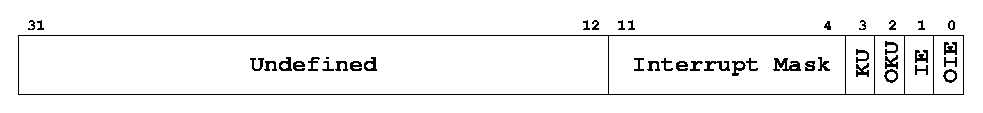
\includegraphics[width=\textwidth]{cctrl.eps}
\caption{\$cctrl - CPU Control Register}
\label{cctrl_pic}
\end{center}
\end{figure}

The CPU control register controls almost all of the functionality
related to the WRAMP exception mechanism. There are three main
sections of this register:

\begin{itemize}
\item Interrupt Enable (IE)
\item Kernel/User Mode (KU)
\item Interrupt Mask
\end{itemize}

\subsubsection{Interrupt Enable}

This flag provides a global interrupt enable. If this location is set
to `\src{0}' then no interrupts can be triggered. This flag
\emph{only} affects external interrupts. There is no way on the WRAMP
processor to disable internal exceptions.

Interrupts that occur while the global interrupt enable is turned off
will be held back. As soon as interrupts are again enabled by writing
a `\src{1}' into this location the interrupt mask will be consulted
to discover if that specific interrupt is enabled. See
Section~\ref{sec:imask} for more information about the interrupt mask.

The CPU will automatically set the IE bit to `\src{0}' whenever an
exception of any type occurs. This prevents the exception handler
from being interrupted by another interrupt.

\subsubsection{Interrupt Mask}
\label{sec:imask}

This provides a way to selectively turn on and off individual external
interrupts. This field has a bit corresponding to each of the eight
possible external interrupts (IRQ0 - IRQ7). Bit 4 of the CPU control
register corresponds to IRQ0, bit 5 to IRQ1 and so on.

The interrupt mask field is only consulted if the global interrupt
enable (IE) flag is set. If an interrupt occurs and the global
interrupt flag is set but the individual interrupt mask is disabled
then the interrupt will be held back. As soon as both the global
interrupt enable and the specific interrupt mask bits are set then the
interrupt will occur.

\subsubsection{Kernel User Mode}

The WRAMP CPU has two modes of operation, kernel and user mode. If
there is a `\src{1}' in the KU bit the CPU is in kernel mode. If
the KU bit is set to `\src{0}' then the CPU is in user mode. 

If the CPU is running in kernel mode it will execute all instructions and
allow access to all areas of memory. If the CPU is running in user
mode programs are not allowed to use any of the three instructions
which deal with the special register file (\src{movsg, movgs, rfe})
and may not be able to access all memory locations. If a program
running in user mode attempts to use one of these instructions, or to
access protected memory the CPU will cause a General Protection Fault
exception.

The CPU will automatically set the KU bit to `\src{1}' whenever an
exception of any type occurs. This allows the exception handler to
operate in kernel mode, allowing it full access to all instructions
and memory locations.

\subsection{\$estat - Exception Status Register}

\begin{figure}[h]
\begin{center}
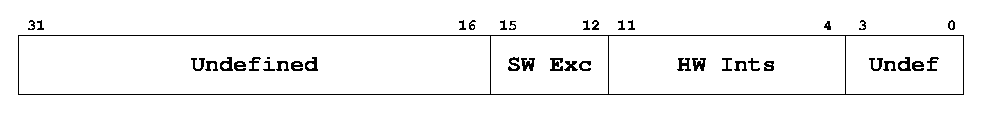
\includegraphics[width=\textwidth]{estat.eps}
\caption{\$estat - Exception Status Register}
\label{estat_pic}
\end{center}
\end{figure}

The exception status register provides the exception handler with the
ability to discover which exceptions caused it to be invoked. The
exception status register has a single bit flag for each external IRQ
line. Bit 4 of the status register corresponds to IRQ0, bit 5 to IRQ 1
and so on. These locations are exactly the same as the locations of
the interrupt mask fields in the CPU control register as described in
Section~\ref{sec:imask}. In addition to the eight external interrupt
sources the status register also provides the status for the four CPU
internal exception sources. 

The full list of all exception sources and their related status
register bit is given in Table~\ref{table:sta_loc}.

Most exception handlers will wish to check which exception caused them
to be called. Provided in Figure~\ref{code:stat_check} is code that
checks if a specific interrupt caused the handler to be called. If any
other interrupt or exception is currently high then the code will call
an old handler to deal with the exception. The code to save the
address of an old handler is given in Figure~\ref{code:evec} and
discussed in Section~\ref{sec:evec}.

\begin{table}[h]
\begin{center}
\begin{tabular}{|l|c|}
\hline
\textbf{Exception source} & \textbf{Bit location} \\
\hline
IRQ0 & 4 \\
\hline
IRQ1 - User Interrupt Button & 5 \\
\hline
IRQ2 - Timer Interrupt & 6 \\
\hline
IRQ3 - Parallel Interrupt & 7 \\
\hline
IRQ4 - Serial Port 1 Interrupt & 8 \\
\hline
IRQ5 - Serial Port 2 Interrupt & 9 \\
\hline
IRQ6 & 10 \\
\hline
IRQ7 & 11 \\
\hline
General Protection Fault Exception & 12 \\
\hline
System Call Exception & 13 \\
\hline
Breakpoint Exception & 14 \\
\hline
Arithmetic Exception & 15 \\
\hline
\end{tabular}
\caption{Exception Status Register Fields}
\label{table:sta_loc}
\end{center}
\end{table}

\begin{figure}[h]
\begin{footnotesize}
\begin{center}
\begin{tabular}{|p{10cm}|}
\hline
\begin{verbatim}
          . . .
  handler:

        # Get the status register
        movsg   $13, $estat

        # Inspect only the bits we are interested in. We want 
        # to check that no bits from the sw exceptions or 
        # hardware exceptions, other than the one we were 
        # expecting, are enabled.
        #
        # This code is looking for an IRQ4 interrupt.
        andi    $13, $13, 0xfef0
         
        # If the result of this is zero then no other 
        # exceptions are enabled so it must be our interrupt
        # that caused us to be called.
        beqz    $13, handle_interrupt 

        # Otherwise there was another exception that has 
        # occurred, so call the old handler
        lw      $13, old_vector($0)
        jr      $13

  handle_interrupt:

        # This is where we deal with the interrupt.
           . . .
\end{verbatim}
\\
\hline
\end{tabular}
\end{center}
\end{footnotesize}
\caption{Checking the Status Register}
\label{code:stat_check}
\end{figure}

\subsection{\$evec - Exception Vector Register}
\label{sec:evec}

When an exception occurs the CPU needs to jump to the exception
handler. The CPU must therefore know what address the exception
handler starts at.

The address of the exception handler is stored in the exception vector
register. The CPU jumps to this location whenever an exception occurs.

If a program is replacing an existing exception handler, but will still
need to call the old handler for certain exceptions, the code must
be careful to save the address of the old exception handler. This
allows the new handler to decide if it will deal with this exception,
and if not, call the old handler.

A section of WRAMP code to save the address of an old exception
handler, load the address of the new handler and save this to the
exception vector is given in Figure~\ref{code:evec}.

\begin{figure}[h]
\begin{footnotesize}
\begin{center}
\begin{tabular}{|p{8cm}|}
\hline
\begin{verbatim}
          . . . 
        # Get the old exception vector
        movsg   $4, $evec
        # And save it
        sw      $4, old_vector($0)

        # Get the address of our handler
        la      $4, handler
        # And put it in the exception vector register
        movgs   $evec, $4

            . . .
	
   handler:
        # The exception handler goes here

            . . .

   old_vector:
        .word   0

\end{verbatim}
%$
\\
\hline
\end{tabular}
\end{center}
\end{footnotesize}
\caption{Saving and Initialising the Exception Vector}
\label{code:evec}
\end{figure}

\subsection{\$ear - Exception Address Register}

An exception routine must be able to return to the point in program code at
which the exception occurred.  To allow this, when an exception occurs the
WRAMP pocessor automatically saves the address of the next instruction
that would have been executed into \reg{ear} - the Exception Address
Register.

When the exception routine has completed its processing, it executes a
Return From Exception, or \src{rfe} instruction. Amongst other things, this
instruction causes a jump to the address contained in \reg{ear}.

In some circumstances an exception routine may wish to know the address at
which the exception was invoked, or may wish to alter the address to which
the \src{rfe} will return. This can be achieved by inspecting and/or modifying
the contents of the \reg{ear}.

\subsection{\$ers - Exception Save Register}

It is vital that an exception routine does not change the contents of the
general purpose registers when it returns to the main program, as changes
may cause the main program to behave in an unpredictable fashion.

However, for the exception handler to determine the cause of the exception,
it requires a general purpose register into which it can copy
\reg{estat}. The WRAMP processor makes general purpose register \reg{13}
available for this by automatically copying it to the Exception Save
Register (\reg{ers}) when an exception occurs. The opposite of this happens
when an \src{rfe} instruction is executed - \reg{ers} is copied into
\reg{13}.

This means that exception handler code must only change \reg{13}.  If
it needs other registers it must save their contents before using
them.  They must then be restored before returning to the main
program.

\section{User Interrupt Button}

The REX board provides a simple method for creating an
interrupt. There is a button located on the front of the case, next to
the reset button labeled ``INTR''. When this button is pressed IRQ1,
the ``User Interrupt Button'', interrupt will be triggered. If this
interrupt is unmasked and the global interrupt enable is turned on in
\src{\$cctrl} an exception will occur.

This button provides a simple way to test an exception handler as it
avoids problems that could be caused by mis-configuration of the I/O
device that is being used to provide the exception.

Like all other REX interrupt sources the user interrupt button needs
to be acknowledged each time an exception occurs. To acknowledge a
``User Interrupt'' you store zero to the address
\src{0x7f000}. Unlike the other I/O devices on the REX board you do
not need to enable or disable the user interrupt button. If IRQ1 is
unmasked in \src{\$cctrl} and interrupts are enabled the button
will cause an exception when pressed.

\section{Using Exceptions}

Writing a program that uses exceptions is best done as a step by step
process. If you attempt to write an entire program that uses exceptions
from start to finish in one hit, then there is a good chance you will never
debug any problems that may arise.

The first thing that you will need when writing your first handler is a
simple program that will run as the main loop of your code. You use this to
ensure that the exception routine is returning to your original code
correctly. A program which reads the value on the switches and writes this
to the seven segment display is ideal. Obviously you should do this in a
polled fashion.

Next you should write a very simple piece of code that will constitute
your exception handler. A suggested program is one which writes a
single character to a serial port. As this code will eventually be run
from inside your exception handler it must transmit this character
using polled I/O.

Test that both of these pieces of code work in a normal environment with no
exceptions. Also ensure that the code which will act as your exception
handler makes use only of \reg{13}.

The next step is to actually enable an interrupt and get the handler
you just wrote to be run. As suggested above the best source for your
first interrupt is the user interrupt button, IRQ1. The things that
you need to do to get this working are:

\begin{itemize}
\item Save the old exception handler address
\item Put the address of your new handler into \src{\$evec}
\item Make sure that there are no old interrupts hanging around by
storing \src{\$0} to the acknowledge register of the device you
will be using. For IRQ1 the acknowledge register is at address
\src{0x7f000}.
\item Configure the CPU control register to enable interrupts. This
takes a number of smaller steps:
\begin{itemize}
\item Get the current value of \src{\$cctrl}
\item Disable all interrupts.
\item Enable the interrupt you wish to use (IRQ1) and set the global
interrupt enable to `\src{1}'. Be careful that you do not alter any
other locations in this register besides the ones specified.
\item Store this value back into \src{\$cctrl}.
\end{itemize}
\end{itemize}


You will need to add some code to the simple exception handler that
you just wrote to make it a complete exception handler. Your exception
handler must start with code to detect if the interrupt is one that
you wish to deal with. Some example code for this is given in
Figure~\ref{code:stat_check}. Beware that you will need to alter this
code so that it checks for the correct interrupt. If you are using the
user interrupt button you should make sure the code checks that only
IRQ1 is high.

Next you must remember to acknowledge the interrupt. If you do not
acknowledge the interrupt then as soon as your exception routine exits
it will be instantly called again. This means you code will be stuck
in an infinite loop, probably printing character after character to
the serial port.

The very final instruction of you exception handler must be an
\src{rfe}. Only use an \src{rfe} instruction in code that you
are sure will only be called as part of an exception handler. If you
use the \src{rfe} instruction when you are not inside an exception
handler you may find your code will get stuck in an infinite loop or
crash.

If this code is now working, then you should have a character appearing
each time you push the user interrupt button as well as the value on the
switches constantly being displayed on the seven segment display. If so,
try altering your code so that you use one of the other I/O devices to
cause exceptions.

\section{Exception Procedure}

What actually happens when an exception occurs? The CPU performs a
number of operations when an exception occurs but they are all pretty
simple. The CPU does the following:

\begin{itemize}
\item Copy the IE bit into the OIE bit
\item Set IE to zero
\item Copy the KU bit into the OKU bit
\item Set KU to one
\item Set the \reg{estat} register to reflect the cause of the exception
\item Copy \reg{13} into \reg{ers}
\item Save the program counter into \reg{ear}
\item Set the program counter to the contents of \reg{evec}
\end{itemize}

At this point the next instruction is fetched. This instruction is the
first instruction of the exception handler and therefore the handler
is now running.

Once the exception handler has finished the final instruction it will
call will be an \src{rfe}. The CPU takes the following steps to
execute an \src{rfe} instruction:

\begin{itemize}
\item Set the IE bit to OIE
\item Set the KU bit to OKU
\item Copy \reg{ers} into \reg{13}
\item Set the program counter to the contents of \reg{ear}
\end{itemize}

This means that the next instruction fetched will normally be the
next instruction of the original code. The IE and KU bits will also
normally be restored to the value they had when the exception occurred.
